%\subsection{Validation of the methodology}

% \subsection{Testing is simulated scenario}\label{sec:synth}
To validate the approach we first devised a simulation, where we performed tests on nine everyday objects, represented as polygonal meshes of (Figure~\ref{fig:meshes}).
\begin{figure}[t]
    \centering
    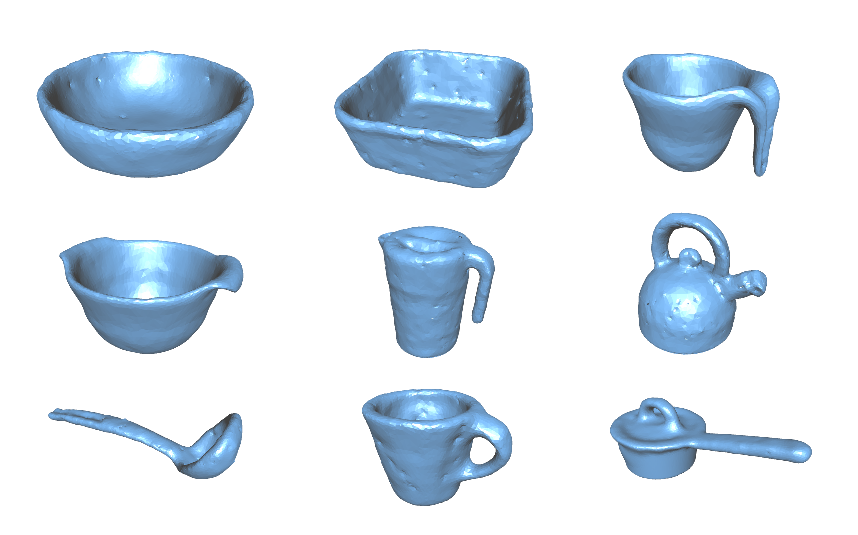
\includegraphics[width=0.95\columnwidth]{meshes.eps}
    \caption{Object meshes used as ground truth for our simulated tests. From top to bottom and from left to right: bowlA, bowlB, containerA, containerB, jug, kettle, spoon, mug and pot.}
    \label{fig:meshes}
\end{figure}
These were obtained using an RGBD sensor and a turntable. They are used as ground truth and to create simulated depth images. Each trial iterated the \textsc{GPAtlasRRT} algorithm, Alg.~\ref{alg:strategy}~in~Sec.~\ref{sec:solution},
until the shape was predicted with desired variance $\mathbb{V}_{\max} = 0.1$.
% find a solution path that defines the best next tactile action to perform, until
The selected tactile actions were simulated using  raycasting. Rays are uniquely defined by a chart center, as pivot point, and its normal, as direction.
Thus we can define ray-mesh intersections as touches, and non intersections as points outside the surface. We adopted three different tactile schemes, thus forming three conditions, for a total of 27 full shape reconstructions. These are as follows.

\begin{asparadesc}
    \item[Random Touch] for the first condition the robot just attempted to touch a random point on the GP manifold. This repeated until the reconstructed shape had a maximum variance of $0.1$. This was our control condition or baseline. Test results are shown in Table~\ref{tab:tests}.
    
    \item[Single Poke] for the second condition we used the \textsc{GPAtlasRRT} by poking the last chart in the path. The convergence criterion was the same as for the random condition. Results in Table~\ref{tab:tests} show a significant reduction
 in the number of tactile actions required to reach the requested shape uncertainty.
 
    \item[Sliding Touch] for the  final condition we  used the full path generated by \textsc{GPAtlasRRT}. Starting from the root chart we made simulated touches and from each one re-interpolated the path toward the next chart. This was repeated until the tip of the atlas branch was reached. As the virtual probe moves across each chart many data points were gathered, in contrast to the single poke or random conditions. We hypothesized this condition would be the best performer in terms of the quality of the reconstructed shape, and in terms of the number of charts traversed. Table~\ref{tab:tests} shows this to be correct.
\end{asparadesc}
%\begin{table}
%    \centering
%    \begin{tabularx}{0.95\columnwidth}{lccccccr}
%        \toprule
%        Object &&& & & Steps && RMSE \\
%        \midrule
%        bowlA &&& & &67 && 0.0025\\
%        bowlB &&& & &38 && 0.0038\\
%        containerA &&&&& 124 && 0.0033\\
%        containerB &&&&& 68 && 0.0062\\
%        jug &&&&& 106 && 0.0027\\
%        kettle &&&&& 98 && 0.0031\\
%        spoon &&&&& 35 && 0.0058\\
%        mug &&&&& 238 && 0.0017\\
%        pot &&&&& 33 && 0.0035\\
%        \midrule
%        \textbf{Mean} &&&&& $\sim$\textbf{90} && \textbf{0.0036}\\
%        \bottomrule
%    \end{tabularx}
%    \caption{Random Touch test results in terms of the required number of actions (Steps) and the Root Mean Squared Error (RMSE) between
%    the predicted shape and the ground truth mesh.}
%    \label{tab:test1}
%\end{table}
%\begin{table}
%    \centering
%    \begin{tabularx}{0.95\columnwidth}{lccccccr}
%        \toprule
%        Object &&& & & Steps && RMSE \\
%        \midrule
%        bowlA &&& & &27 && 0.0023\\
%        bowlB &&& & &18 && 0.0036\\
%        containerA &&&&& 20 && 0.0035\\
%        containerB &&&&& 19 && 0.0043\\
%        jug &&&&& 20 && 0.003\\
%        kettle &&&&& 17 && 0.0032\\
%        spoon &&&&& 10 && 0.0055\\
%        mug &&&&& 28 && 0.0020\\
%        pot &&&&& 12 && 0.0032\\
%        \midrule
%        \textbf{Mean} &&&&& $\sim$\textbf{19} && \textbf{0.0034}\\
%        \bottomrule
%    \end{tabularx}
%    \caption{Single Poking test results in terms of the required
%    number of actions (Steps) and the Root Mean Squared Error (RMSE) between
%    the predicted shape and the ground truth mesh.}
%    \label{tab:test2}
%\end{table}
%\begin{table}
%    \centering
%    \begin{tabularx}{0.95\columnwidth}{lccccccr}
%        \toprule
%        Object & & &&& Steps && RMSE \\
%        \midrule
%        bowlA &&& & &8 && 0.0015\\
%        bowlB & &&& &5 && 0.0028\\
%        containerA &&&&& 11 && 0.0028\\
%        containerB &&&&& 8 && 0.0026\\
%        jug &&&&& 9 && 0.0025\\
%        kettle &&&&& 9 && 0.0029\\
%        spoon &&&&& 8 && 0.0031\\
%        mug &&&&& 12 && 0.0018\\
%        pot &&&&& 6 && 0.0028\\
%        \midrule
%        \textbf{Mean} &&&&& $\sim$\textbf{8} && \textbf{0.0025}\\
%        \bottomrule
%    \end{tabularx}
%    \caption{Sliding Touch test results in terms of the required
%    number of actions (Steps) and the Root Mean Squared Error (RMSE) between
%    the predicted shape and the ground truth mesh.}
%    \label{tab:test3}
%\end{table}

\begin{table}
    \centering
    \begin{tabular}{|l|c|r|c|r|c|r|} \hline
        & \multicolumn{2}{|c|}{Random Poke} & \multicolumn{2}{c|}{Single Poke} & \multicolumn{2}{c|}{Sliding}\\
        \hline
        Object & Steps & RMSE & Steps & RMSE & Steps & RMSE\\
        \hline
        bowlA & 67 & 0.0025 & 27 & 0.0023 &8 & 0.0015\\
        bowlB & 38 & 0.0038 &18 & 0.0036 & 5 & 0.0028\\
        containerA & 124 & 0.0033 & 20 & 0.0035 & 11 & 0.0028\\
        containerB & 68 & 0.0062 & 19 & 0.0043 & 8 & 0.0026\\
        jug & 106 & 0.0027 & 20 & 0.003 & 9 & 0.0025\\
        kettle & 98 & 0.0031 & 17 & 0.0032 & 9 & 0.0029\\
        spoon & 35 & 0.0058 & 10 & 0.0055 & 8 & 0.0031\\
        mug & 238 & 0.0017 & 28 & 0.0020 & 12 & 0.0018\\
        pot & 33 & 0.0035 & 12 & 0.0032 & 6 & 0.0028\\
        \hline
        \textbf{Mean} & $\sim$\textbf{90} & \textbf{0.0036} & $\sim$\textbf{19} & \textbf{0.0034} & $\sim$\textbf{8} & \textbf{0.0025}\\
        \hline
    \end{tabular}
    \caption{Simulated results for all three conditions in terms of the required number of actions (Steps) and the Root Mean Squared Error (RMSE) between the predicted shape and the ground truth mesh.}
    \label{tab:tests}
\end{table}

The three experiments clearly show the superiority of the single poke and sliding touch methods in terms of number of required steps
and in terms of quality of the produced mesh. As a final benchmark, Table~\ref{tab:comp} summarizes the comparison
between the test methods and Fig.~\ref{fig:shapecomp} shows some  of the \textsc{GPAtlasRRT} Sliding Touch reconstructed shapes with
the ground truth meshes next to them.\footnote{Additionally, we recorded videos of the shape reconstructions, see \texttt{goo.gl/4GKYTp}.}
\begin{table}
    \centering
    \begin{tabular}{|l|c|r|}
        \hline
        Tests  & Mean Steps & Mean RMSE \\
        \hline
        Random Touch & 90 & 0.0036\\
        Single Poking &19 & 0.0034\\
        Sliding Touch &8 & 0.0025\\
        \hline
    \end{tabular}
    \caption{Overall comparison: GPAtlasRRT with Sliding Touch outperforms in terms
    of efficiency and accuracy.}
    \label{tab:comp}
\end{table}

\begin{figure}[htb]
    \centering
    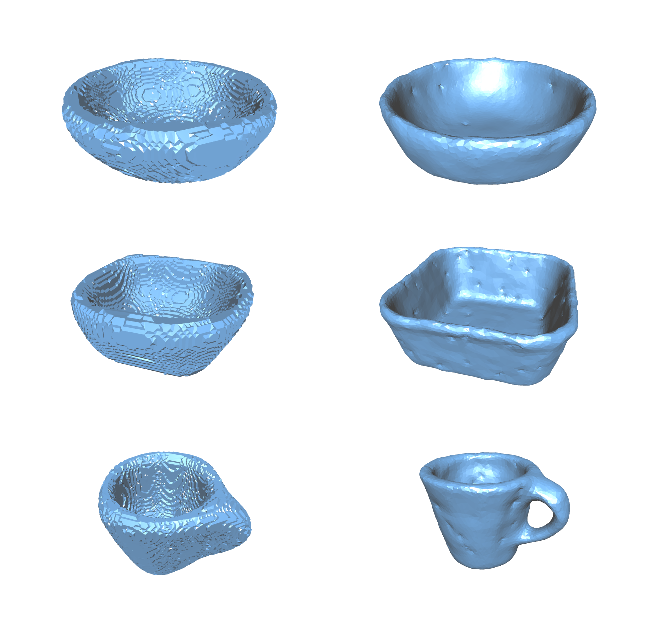
\includegraphics[width=0.95\columnwidth]{comparison.eps}
    \caption{Comparison of reconstructed shapes (left) with the ground truth meshes (right), obtained with our GPAtlasRRT via the Sliding Touch method.}
    \label{fig:shapecomp}
\end{figure}


\subsection{A real robot experiment}
\label{sec:real}

This section provides an empirical evaluation of our proposed method on a real robotic platform. Our setup differs from the simulated environment in the following ways: i) we only demonstrated the Single Poke approach (described at the beginning of this section), and ii) the object is not handed to the robot, but held on the table via a clamp. The latter implies that we only use Boris' left arm (equipped with the intrinsic tactile sensor) to carry out the experiments. This choice is justified by the fact that, in this setup, the robot can reach and touch a larger proportion of the object's surface. Figure~\ref{fig:boris} shows the setup.

The empirical data has been generated as follows. Boris takes a snapshot of the environment via a depth camera attached to its chest. The acquired point cloud is then filtered such that to remove all the points that do not belong to the object. The point cloud describing the object is passed as input to the GP and the GPAtlasRRT procedure is started. We demonstrated the method on three objects: a jug, a dustpan, and a plate. 

\begin{figure}[htb]
    \centering
    \includegraphics[width=0.5\columnwidth]{Boris_jug002_adjust.png}
    \caption{Real experimental setup. Boris explores an object fixed on the table.}
    \label{fig:boris}
\end{figure}

\section{A real tactile exploration}
\label{sec:vito}

The purpose of this trial was to illustrate a complete robot implementation of Algorithm \ref{alg:solution}. As mentioned in Section~\ref{sec:gpatlasrrt_tactile_exploration}, we don't implement a re-grasping manoeuvre to overcome hand-induced occlusions.\footnote{The implementation is mixed open-source \texttt{github.com/CentroEPiaggio/pacman-DR54}, heavily-based on the Robot Operating System \cite{ROS}. The GPAtlasRRT (Algorithm \ref{alg:strategy}) is a submodule \texttt{github.com/pacman-project/gaussian-object-modelling}. As with the simulated results, we present an accompanying video \texttt{https://goo.gl/4GKYTp}.} The technical details are now given.

In this scenario, we employ our Vito and Boris robots. These are bimanual robots equipped with 2 KUKA LWR 4+, one Pisa/IIT SoftHand~\cite{Catalano2014Adaptive} as one end-effector, and the intrinsic tactile sensor configuration as introduced by \cite{Rosales2014Active}. We start a trial by handing the robot an object. Afterwards, the object is segmented with the help of the recently developed IMU-based glove by \cite{Santaera2015Lowcost} to measure the hand configuration, and we remove the entire robot body from the scene. Other typical filters such as pass-through and down-sampling were applied to speed-up the overall pipeline. The acquired cloud contained an incomplete view of the object and constituted the initial training data for the Gaussian process, namely $\mathcal{S}^0$. Fig. \ref{fig:real} shows the initial model. Then a sequence of touches was performed. The grasping hand necessarily prevents full completion of the model, so an additional terminating condition is used.\footnote{This is a threshold for a number of failed consecutive attempts to execute a touch, and models the fact that it is not possible to touch areas occluded by the hand.} 

The setup included three standard personal computers, where one was dedicated to the GPAtlasRRT strategy, one acted as the decision-maker and the last was the hardware server. Most time is consumed in the computation of the explicit form of the object for collision-avoidance motion planning. Suggested tactile actions were checked for an inverse kinematics solution. If this failed another touch candidate was requested. Note that both the GPAtlasRRT strategy and the motion planner are probabilistic, and their combination in some cases led to the planner being trapped in a local-minima.

\begin{figure}
\centering
%\mbox{
  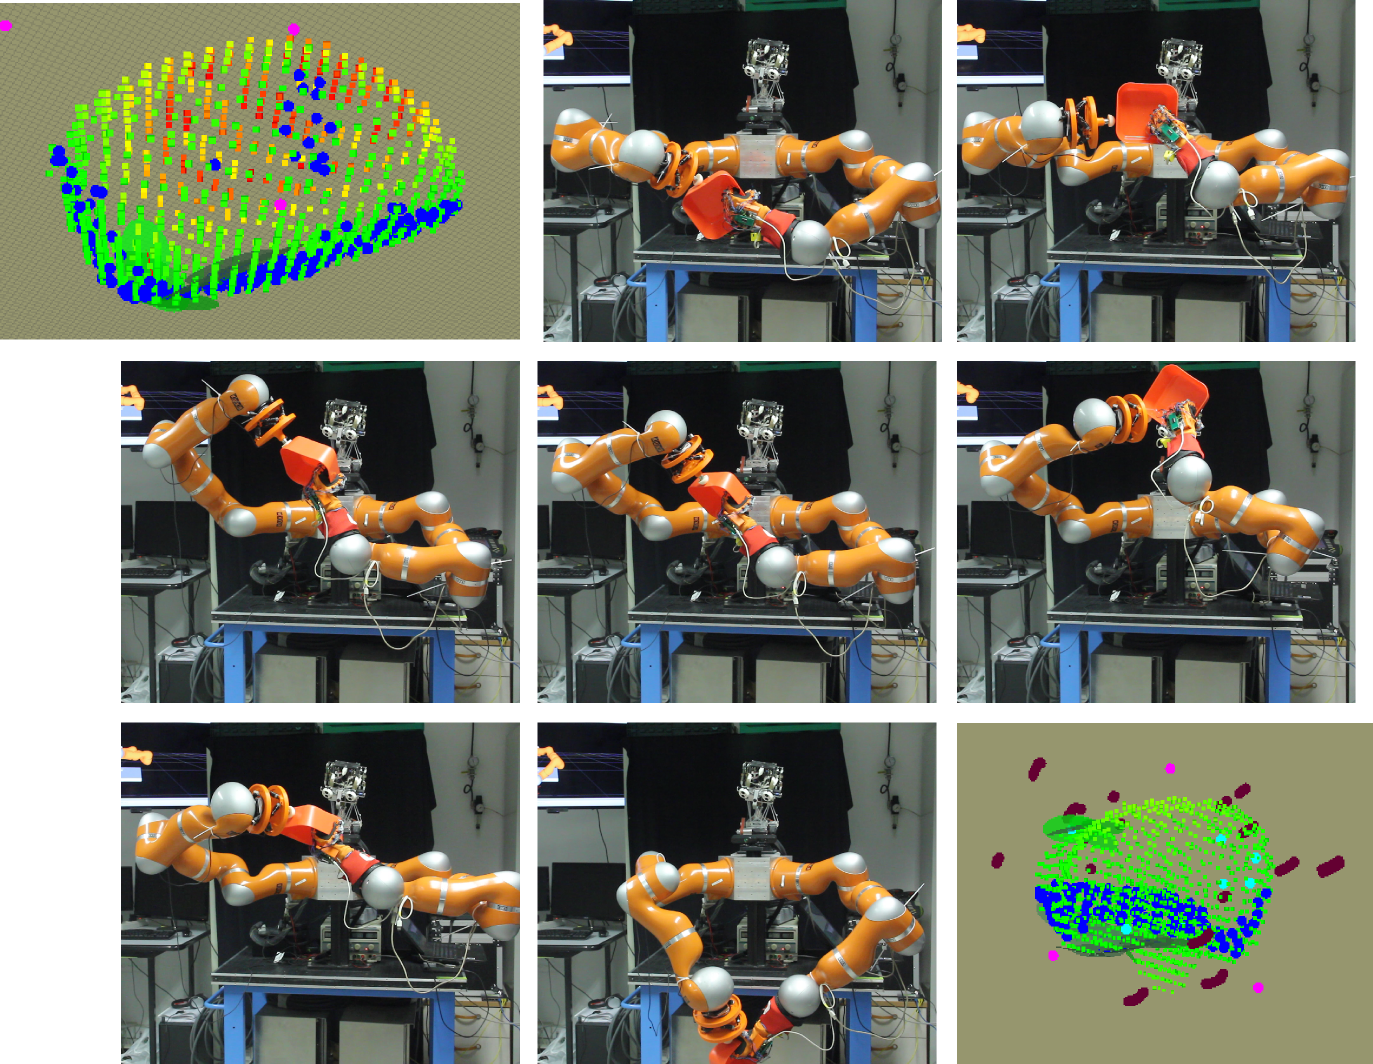
\includegraphics[width=0.9\linewidth]{real_shots.png}
%}
\caption{Our Vito robot performs a tactile exploration action using the proposed GPAtlasRRT strategy. The per-point colour code  is the same as in Fig.~\ref{fig:setup_solution}}
\label{fig:real}
\end{figure}